\ofsubsection{Siege of Dollet}
%
\ofquote{
"The elite mercenary force, SeeD! Learn from them, obey their
commands and accomplish the mission. Prove yourselves worth of
becoming a member of SeeD."
}{Headmaster Cid}
%
\vfill
%
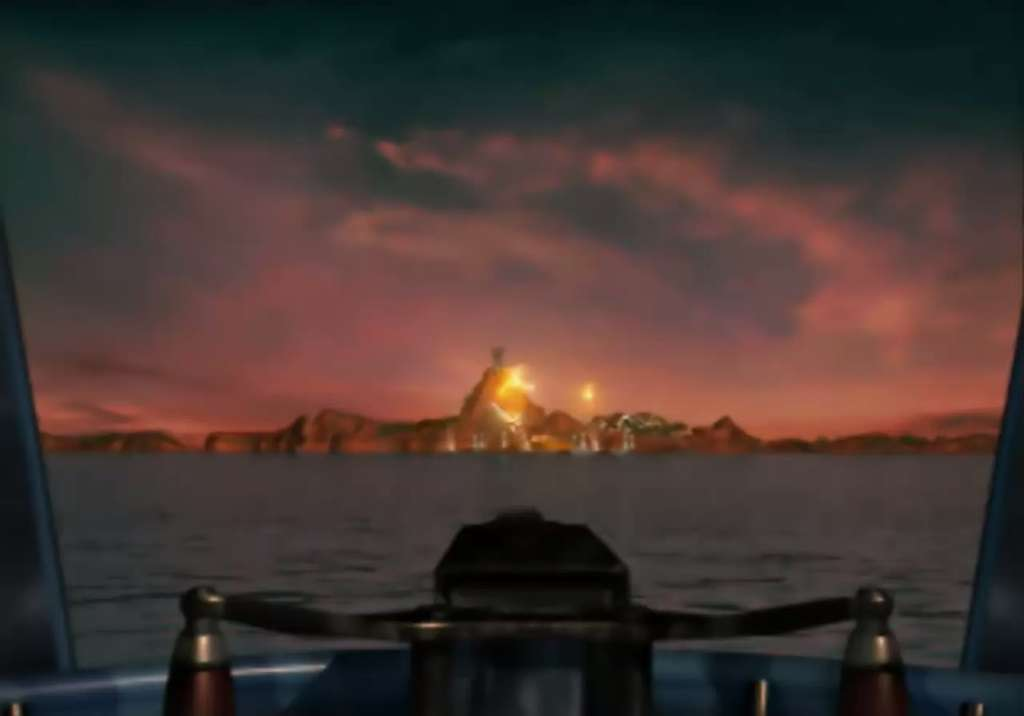
\includegraphics[width=\columnwidth]{./art/siegeofdollet/island.jpg}
%
\vfill
%
\accf{Siege of Dollet} is a pre-prepared adventure that can be completed in a single session.
The players take the role of students who are training to become members of an elite mercenary group called SeeD. 
They can either use the pre-made character sheets at the end of this document or use them as examples to create their
own characters.
You as the GM take the role of their instructor to guide the students through their final exam.
%
\vfill
%
\ofquote{"Sounds boring. So what you're saying is, we do all the little, dirtywork..."}{Seifer}\\\\
%
Good morning, instructor.
My name is Xu and I will provide you with as much intel throughout the day as I can.
You and all of your students that will be taking today's exam should currently be on one of our assault gunboats that are on the way to Dollet.
Remember, your job is only to guide the students, we want to see if they can prove themselves worthy of becoming SeeD.
As such you will stay on this boat during the mission, but you can talk to the students at any time using the earpiece through which you are also hearing me right now.
Make sure that everyone makes it out alive!
%
\vfill
%
Concerning the mission:
the SeeD squads have been hired by the Dollet Parliament to defend them against a siege from the Galbadian army.
Your students form squad B and are tasked with clearing out and holding the inner city of Dollet.
We have intel that the majority of the Galbadian army have moved elsewhere, where the rest of the SeeD will be ambushing them. 
Make sure to go over these mission details with the students before you arrive. 
Oh, and don't forget to name one of them as the squad leader.
%
\newpage
%
\ofquote{"Look out, it's SeeD!"\\}{Galbadian Soldier}
%
\vfill
%
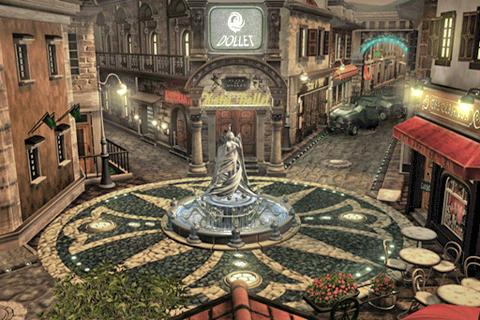
\includegraphics[width=\columnwidth]{./art/siegeofdollet/dollet.jpg} 
%
\vfill
%
You should soon arrive at Lapin Beach before Dollet.
The Galbadians have built up some defenses at the shore, but those should be no match for our gun boats.
After the beach is clear, squad B should leave the boat to start the exam.
They can move up the stairs to their left and from there follow the alley into the town square.
I can see 3 Galbadian soldiers guarding the town center, it could be more though.
Each student that passes a DC~7 check should be able to notice them as well.
Let's see how they handle themselves.
%
\vfill
%
\ofmonster{Galbadian Soldier}{1}{
\includegraphics[width=0.15\columnwidth]{./art/siegeofdollet/gsoldier.png}}
{
	HP: & \hfill 12 & MP: & \hfill 0\\
	STR: & \hfill 1 & DEF: & \hfill 0 \\
	MAG: & \hfill 0 & RES: & \hfill 0 \\
	AGI: & \hfill 2 & Size: & \hfill M\\
}
{\accf{Machine Gun}: 1d DMG, 3u range \hfill \accf{Drops:} 100 Gil}{}
%
\vfill
%
The Galbadians sure aren't making it easy for them.
They are using the fountain as a cover to avoid going into melee.  
After defeating these soldiers, squad B just needs to make sure that the inner city stays clear. 
If they decide to look around they might find some useful things like Potions.
There is also a lone dog wandering around, poor guy probably got lost in this mess.
It has been an hour now and I think the students are getting bored. 
Looks like everything is... wait a second.
I can see a large group of Galbadians moving quickly towards the town square!
Squad B needs to hide immediately! 
Hmm... it doesn't look like the soldiers want to retake the inner city, they are going somewhere else.
What are they up to?
%
\vfill
%
They are moving towards the mountain path, but there is nothing up there, except that old radio tower I think.
I don't know if the students understood what is going on, but the dog sure has.
Well at least he is howling at the mountain.
What are your orders instructor?
Remember, squad B needs to hold the inner city, but those Galbadians are clearly up to something.
I hope the students will follow your orders...
%
\clearpage
%
\ofquote{"WEDGE! Where were you!? No pay for you this month!"}{Major Biggs}
%
\vfill
%
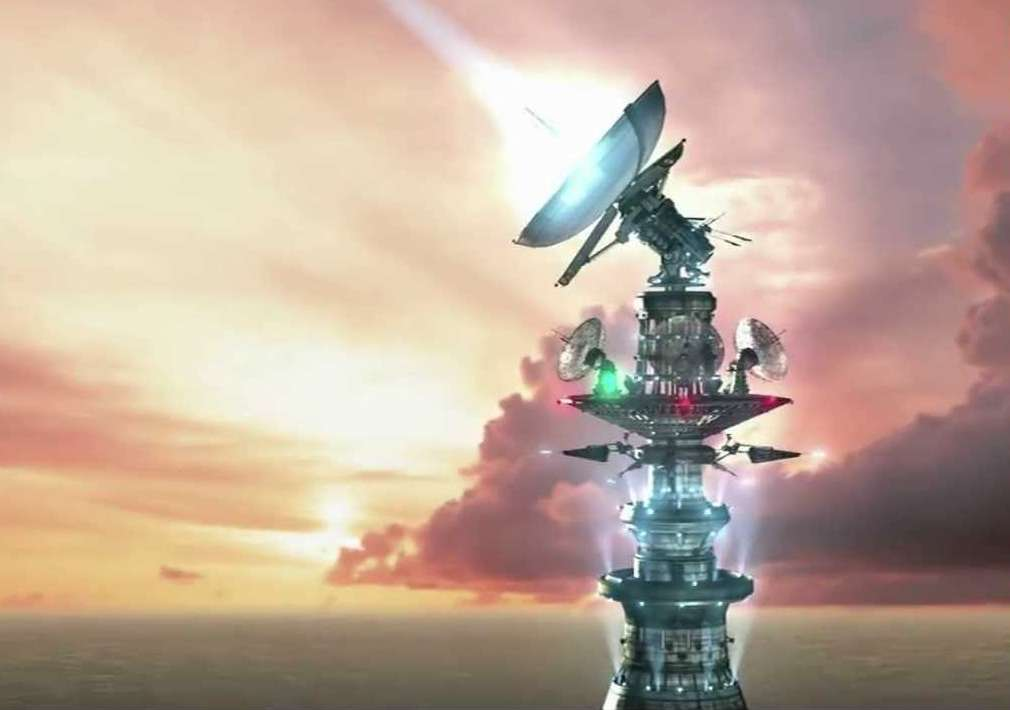
\includegraphics[width=\columnwidth]{./art/siegeofdollet/tower.jpg}
%
\vfill
%
Squad B is also making its way up the mountain, I hope they make sure to stay undetected.
There are a few of Dollet's soldiers stationed on the path, but the Galbadians are cutting through them like butter.
Still, they are suffering many casualties on the way, I think only 2 Galbadians have actually made it to the tower.
Squad~B should be able to reach the tower without any issues.
Looks like they have almost reached the mountain top.
The Galbadians have meanwhile made their way up to the platform of the radio tower and I think they are making repairs.
At least they have managed to reactivate the radio tower.
That also means the students can take the elevator on the ground floor to reach them.
%
\vfill
%
\ofmonster{Major Biggs}{2}{
\includegraphics[width=0.22\columnwidth]{./art/siegeofdollet/biggs.png}}
{
	HP: & \hfill 28 & MP: & \hfill 24\\
	STR: & \hfill 2 & DEF: & \hfill 2 \\
	MAG: & \hfill 1 & RES: & \hfill 1 \\
	AGI: & \hfill 2 & Size: & \hfill M\\
}
{\accf{Machine Gun}: 1d DMG, 3u Range \hfill \accf{Drops:} 300 Gil}
{
	\mspell{Thunder}{4}{0r}{Single}{3u}{You deal 2d lightning damage to the target.}{\lightning}	
	\mtech{Rush}{3}{0r}{Single}{Weapon}{Make an Attack against the target. If you hit, you push him back by 1u on top of the damage dealt.}{}	
}
%
\vfill
%
\ofmonster{Wedge}{2}{
\includegraphics[width=0.15\columnwidth]{./art/siegeofdollet/gsoldier.png}}
{
	HP: & \hfill 22 & MP: & \hfill 16\\
	STR: & \hfill 2 & DEF: & \hfill 1 \\
	MAG: & \hfill 1 & RES: & \hfill 1 \\
	AGI: & \hfill 3 & Size: & \hfill M\\
}
{\accf{Sword}: 1d DMG \hfill \accf{Drops:} 200 Gil}
{\mspell{Fire}{4}{0r}{Single}{3u}{You deal fire damage to the target.}{\fire}	}
%
\newpage
%
I can now see squad B on the top of the tower, confronting the 2 Galbadian soldiers, one of them seems to be their leader. 
I think I have understood their strategy: they are trying force the students to the edge of the platform to knock them off the tower.
Should that happen, I think the students should be able to hold onto something if they pass a DC 5 check and another squad member can then spend an action to pull them back up. 
Anyway, the Galbadians do not seem very competent otherwise.
And... Squad B was able to neutralize the enemy!
We have also just received an important order:
all squads are to retreat back to Lapin Beach immediately, our boats depart in half an hour.
Squads that do not make it to the shore in 30 minutes will get left behind!
I think squad~B can... wait, what the kupo is THAT?!\\\\
%
\vfill
%
\ofmonster{X-ATM092}{4}{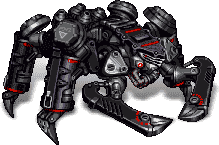
\includegraphics[width=0.3\columnwidth]{./art/siegeofdollet/mech.png}}
{
	HP: & \hfill ??? & MP: & \hfill 80\\
	STR: & \hfill 2 & DEF: & \hfill 3 \\
	MAG: & \hfill 0 & RES: & \hfill 1 \\
	AGI: & \hfill 4 & Size: & \hfill L\\
}
{\accf{Claw}: 2d DMG, 2u Range}
{
	\mtech{Ray Bomb}{5}{0r}{2u}{5u}{You deal 2d fire damage to all enemies inside the target area.}{\fire}	
	\mtech{Arm Crush}{3}{0r}{Single}{Weapon}{The target makes a DC 8 check and suffers 2d damage and Immobile for 1 round upon failure}{\immobile}	
}
%
\vfill
%
I don't know where the Galbadians got that thing from, but it is running after the students.
It looks like the thing will overtake all squad members that fail to pass a DC 8 check, I hope the rest do not leave them behind.
There is no way squad B can destroy it in combat, especially if they want to make it in time.
But there is another way: if they attack its legs a few times, it will collapse and begin to repair itself, which gives them time to run.
It's one of the known common vulnerabilities in Galbadian machines, so it should work. 
Still, I think they will have to fight the thing at least twice before they reach the shore.
But maybe they can also come up with something to stop it, a blockade or distraction?
%
\vfill
%
Squad B is now running through Dollet and closing in on the beach, but the machine is still following them.
Instructor, there is a powerful machine gun mounted to the deck of your boat, it should melt through it! 
...I think you got it, great job! 
Squad B has also boarded the boat, so you are ready to go!
Phew... that was close, I hope everyone has made it out alive.
So what do you think Instructor, how did the students do on the exam?
Which ones should we promote to SeeD?
%
\clearpage